\documentclass{article} % Default font size and left-justified equations
% \documentclass{book}

\usepackage[
  margin=0.7in,
  % includefoot,
  % footskip=30pt,
]{geometry}

\usepackage{natbib}
\usepackage{enumitem}
\usepackage{amsmath,amsfonts}
\usepackage{graphicx}
\usepackage{framed}
\usepackage{subcaption}
\usepackage[T1]{fontenc}%
\usepackage[utf8]{inputenc}%
\usepackage{mathrsfs}%
\usepackage{amssymb}%
\usepackage{amsthm}%
\usepackage{graphicx}
\usepackage{hyperref}
\usepackage{environ}
\usepackage{framed}
\usepackage{mdframed} 
\usepackage{wrapfig} 
\usepackage{booktabs}
\usepackage{tabularx} 
\usepackage{array}
\usepackage[font=small]{caption} 
\usepackage{xspace}  
\usepackage[osf,sc]{mathpazo}
\usepackage{pbox}
\usepackage{listings}
\usepackage{tikz}
\usepackage{bm}
\usepackage[strict]{changepage}
\usepackage{mleftright}
\usepackage{appendix}%
\usepackage[all]{xy} 
\setcounter{tocdepth}{3}
\setcounter{secnumdepth}{3}
\usepackage[ruled,vlined]{algorithm2e}
\usepackage{framed}
\usepackage{wrapfig}
\usepackage{pythonhighlight}
\usepackage{tikz}
\usetikzlibrary{arrows}
\usetikzlibrary{arrows.meta}
\usetikzlibrary{shapes.geometric}
\usetikzlibrary{positioning, arrows, automata, calc}
\usepackage{transparent}
\usepackage[many]{tcolorbox}
\usepackage{tikz}
\usetikzlibrary{shapes.geometric}
\usetikzlibrary{positioning, arrows, automata, calc}

\newtcolorbox[]{your_solution}[1][]{
    % breakable,
    enhanced,
    nobeforeafter,
    colback=white,
    title=Your Answer,
    sidebyside align=top,
    box align=top,
    #1
}
\newcommand{\mybox}[1]{
\noindent
\fbox{\parbox{0.955\textwidth}{%
\noindent\texttt{#1}
}
}
}

\newcommand{\filler}{ . . . . . }
\newcommand{\choice}{\hspace{0.5cm}$\square$}
\newcommand{\identity}{\mathbf{I}} 
\newcommand{\paran}[1]{\left( #1 \right)}

%% PLEASE USE THESE MACROS WHEN WRITING THE SOLUTIONS 
\newcommand{\solution}[1]{\textcolor{blue}{Answer: \em #1}
} % show
%\newcommand{\solution}[2]{#2} % hide

\newcommand{\extracredit}{{\color{purple}\textbf{Extra Credit:}}}

\newcommand{\additionalNotes}{
\noindent\textbf{How to hand in your written work:} via MyClasses.  \\ 


\noindent\textbf{Collaboration:} Make certain that you understand the course collaboration policy, described on the course website. 
You may discuss the homework to understand the problems and the mathematics behind the various learning algorithms, but you are \textcolor{red}{\textbf{not allowed to share problem solutions with any other students. You must write the solutions \textbf{individually}}}. \\ 

\noindent\textbf{Typesetting:} 
We strongly recommend typesetting your homework, especially if you have sloppy handwriting. 
% We recommend using LaTeX, but you are welcome to use whatever program and/or markup language you like. 
We will provide a LaTeX template for homework solutions. Type your answers into the corresponding solution field under each question.
}

\title{ \Large COSC490LLMs }
\date{
\normalsize Name: Dustin O'Brien    \\ 
Collaborators, if any: None \\ 
Sources used for your homework, if any: Currently None
}

\newcommand{\todo}{\textcolor{blue}{\textbf{TODOs}}}



\usepackage{macros}

\usepackage{listings}
\usepackage{xcolor}

\definecolor{codegreen}{rgb}{0,0.6,0}
\definecolor{codegray}{rgb}{0.5,0.5,0.5}
\definecolor{codepurple}{rgb}{0.58,0,0.82}
\definecolor{backcolour}{rgb}{0.95,0.95,0.92}

\lstdefinestyle{mystyle}{
    backgroundcolor=\color{backcolour},   
    commentstyle=\color{codegreen},
    keywordstyle=\color{magenta},
    numberstyle=\tiny\color{codegray},
    stringstyle=\color{codepurple},
    basicstyle=\ttfamily\footnotesize,
    breakatwhitespace=false,         
    breaklines=true,                 
    captionpos=b,                    
    keepspaces=true,                 
    numbers=left,                    
    numbersep=5pt,                  
    showspaces=false,                
    showstringspaces=false,
    showtabs=false,                  
    tabsize=2
}

\lstset{style=mystyle}

\author{
\Large
Homework 5: Transformers/Self-Attention 
}


\begin{document}

\maketitle

This assignment focuses on basic understanding of Transformers for language modeling. We will also touch upon Tokenization.  

\noindent\fbox{
    \parbox{\textwidth}{
        \textbf{Homework goals:} After completing this homework, you should be comfortable with: 
        \begin{itemize} 
            \item thinking about Self-Attention module and implementing a simple Transformer language model. 
            % \item how tokenization works and simple implementation of it. 
        \end{itemize}
    }
}

\vspace{0.5cm}


%\additionalNotesTeamUpTwo%


\clearpage



\section{Concepts, intuitions and big picture}
Each question might have multiple correct answers.  (Check all that apply).

\begin{enumerate}
    
    \item Which of these types of models would you use for completing prompts with generated text? \\ 
        \hspace{1cm}\choice{} An encoder model \\ 
        \hspace{1cm}\checkmark{} A decoder model \\ 
        \solution{}
    \item Which of these types of models would you use for classifying text inputs according to certain labels? \\ 
        \hspace{1cm}\checkmark{} An encoder model \\ 
        \hspace{1cm}\choice{} A decoder model \\ 
        \solution{}
    \item To which of these tasks would you apply a many-to-one RNN architecture? \\ 
        \hspace{1cm}\choice{} Speech recognition (input an audio clip and output a transcript) \\ 
        \hspace{1cm}\checkmark{} Sentiment classification (input a piece of text and output a 0/1 to denote positive or negative sentiment) \\ 
        \hspace{1cm}\checkmark{} Gender recognition from speech (input an audio clip and output a label indicating the speaker’s gender) \\ 
        \solution{}
    \item What possible source can the bias observed in a model have?  \\ 
        \hspace{1cm}\checkmark{} The model is a fine-tuned version of a pretrained model and it picked up its bias from it. \\ 
        \hspace{1cm}\checkmark{} The data the model was trained on is biased. \\ 
        \hspace{1cm}\checkmark{} The metric the model was optimizing for is biased. \\ 
        \solution{}
    
    \item How many dimensions does the tensor output by a decoder Transformer model have, and what are they? \\ 
        \hspace{1cm}\choice{} 2: The sequence length and the batch size \\ 
        \hspace{1cm}\choice{} 2: The sequence length and the hidden size \\ 
        \hspace{1cm}\checkmark{}  3: The sequence length, the batch size, and the hidden size \\ 
        \solution{}
    \item You are training an RNN language model. At the $t$th time step, what is the RNN doing? Choose the best answer. \\ 
        \hspace{1cm}\choice{}  Estimating P($y_{1}, y_2, ..., y_{t-1}$) \\ 
        \hspace{1cm}\choice{}  Estimating P($y_1$) \\ 
        \hspace{1cm}\checkmark{}  Estimating P($y_t | y_1, y_2, ..., y_{t-1}$) \\ 
        \hspace{1cm}\choice{}  Estimating P($y_t | y_1, y_2, ..., y_t$) \\ 
    \solution{}
    
    \item You are training an RNN, and find that your weights and activations are all taking on the value of \texttt{NaN} (``Not a Number''). Which of these is the most likely cause of this problem? \\ 
        \hspace{1cm}\choice{} Vanishing gradient problem. \\ 
        \hspace{1cm}\checkmark{} Exploding gradient problem. \\ 
        \hspace{1cm}\choice{} ReLU activation function g(.) used to compute g(z), where z is too large. \\ 
        \hspace{1cm}\choice{} Sigmoid activation function g(.) used to compute g(z), where z is too large. \\ 
        \solution{}

    \item You're done training an RNN language model. You're usig it to sample random sentences as follows. What are you doing at each time step $t$? \\ 
        \hspace{1cm}\choice{}  (i) Use the probabilities output by the RNN to pick the highest probability word for that time-step as $y_t$. (ii) Then pass the ground-truth word from the training set to the next time-step. \\ 
        \hspace{1cm}\choice{}  (i) Use the probabilities output by the RNN to randomly sample a chosen word for that time-step as $y_t$. (ii) Then pass the ground-truth word from the training set to the next time-step. \\ 
        \hspace{1cm}\choice{}  (i) Use the probabilities output by the RNN to pick the highest probability word for that time-step as $y_t$. (ii) Then pass this selected word to the next time-step. \\ 
        \hspace{1cm}\checkmark{}  (i) Use the probabilities output by the RNN to randomly sample a chosen word for that time-step as $y_t$. (ii) Then pass this selected word to the next time-step.

        \solution{}

    
    \item  You have a pet crab whose mood is heavily dependent on the current and past few days' weather. 
        You've collected data for the past 42 days on the weather, which you represent as a sequence as $x_1, ..., x_{42}$. 
        You've also collected data on your crab's mood, which you represent as $y_1, ..., y_{42}$. You’d like to build a model to map from $x \rightarrow y$. Should you use a Unidirectional RNN or Bidirectional RNN for this problem? \\ 
        \hspace{1cm}\choice{} Bidirectional RNN, because this allows the prediction of mood on day $t$ to consider more information. \\ 
        \hspace{1cm}\choice{} Bidirectional RNN, because this allows backpropagation to compute more accurate gradients. \\ 
        \hspace{1cm}\checkmark{} Unidirectional RNN, because the value of $y_t$ depends only on $x_1, ...,x_t$ but not on $x_{t+1},...,x_{42}$
        \hspace{1cm}\choice{} Unidirectional RNN, because the value of $y_t$ depends only on $x$, and not other days' weather. \\ 
        \solution{}
    \item Consider this encoder-decoder model. 
        \begin{figure}[h]
            \centering
            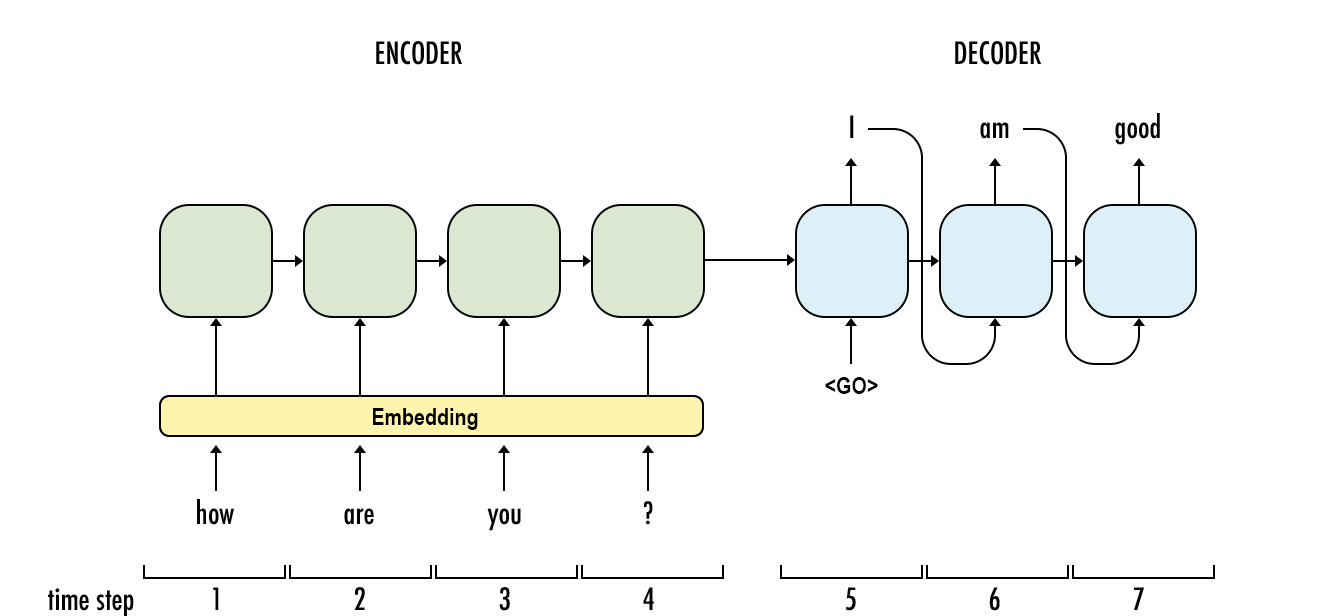
\includegraphics[scale=0.30]{figures/enc-dec.png}
            % \caption{Caption}
            % \label{fig:my_label}
        \end{figure}
        This model is a ``conditional language model'' in the sense that the encoder portion (shown in green) is modeling the probability of the input sentence $x$.\\
        \hspace{1cm}\choice{} True \hspace{1cm}\checkmark{} False \\
        \solution{}
    \item Compared to the RNN-LMs and fixed-window-LMs, we expect the attention-based LMs to have the greatest advantage when: \\ 
        \hspace{1cm}\checkmark{} The input sequence length is large. \\ 
        \hspace{1cm}\choice{} The input sequence length is small. \\
        \solution{}
    \item What is a model head? \\ 
        \hspace{1cm}\choice{} A component of the base Transformer network that redirects tensors to their correct layers \\ 
        \hspace{1cm}\choice{} Also known as the self-attention mechanism, it adapts the representation of a token according to the other tokens of the sequence \\ 
        \hspace{1cm}\checkmark{} An additional component, usually made up of one or a few layers, to convert the transformer predictions to a task-specific output  \\ 
        \solution{}
    \item  What are the techniques to be aware of when batching sequences of different lengths together? \\ 
        \hspace{1cm}\checkmark{} Truncating 
        \hspace{1cm}\choice{} Returning tensors
        \hspace{1cm}\checkmark{} Padding
        \hspace{1cm}\checkmark{} Attention masking \\ 
        \solution{}


\end{enumerate}

\newpage


\newcommand{\xv}{\mathbf{x}}
\newcommand{\yv}{\mathbf{y}}
\newcommand{\Wv}{\mathbf{W}}
\newcommand{\Xv}{\mathbf{X}}
\newcommand{\Yv}{\mathbf{Y}}
\newcommand{\hv}{\mathbf{h}}
\newcommand{\ov}{\mathbf{o}}
\newcommand{\zv}{\mathbf{z}}
\newcommand{\gv}{\mathbf{g}}



\clearpage
\begin{wraptable}[12]{r}{5.5cm}
 \vspace{-1cm}
 \noindent\fbox{%
 % \begin{framed}
 \parbox{5.5cm}{%
 \scriptsize
In Transformers, patterns align and flow,\\
Each token learns where meanings grow.\\
Context builds with layers deep,\\
A dance of words, a bond to keep.\\

And on this day, as time moves on,\\
Self-attention still makes us strong.\\
Not just in models, cold and bright,\\
But in our hearts, it sheds new light.\\

To know ourselves, we must attend,\\
To every thought, each truth we send.\\
With care and kindness, let us see,\\
The love within, wild and free.\\

So as this day of life unfolds,\\
Let self-reflection make us bold.\\
May we embrace both heart and mind,\\
And in their depths, true love we find.\\

\hspace{1.8cm}--ChatGPT Feb 25, 2025
% \end{framed}
}
}
\end{wraptable}
\section{Self-Attention and Transformers}

Recall that the transformer architecture uses scaled dot-product attention to compute \textit{attention weights}:
\begin{align*}
    \boldsymbol{\alpha}^{(t)}  =  \text{softmax} \left( \frac{\textbf{q}_t \textbf{K}^\top }  {\sqrt{h}} \right) \in [0, 1]^n 
\end{align*}
The resulting embedding in the output of attention at position $t$ are: 
$$\text{Attention}(\textbf{Q}, \textbf{K}, \textbf{V})_t = \sum_{t'=1}^n  \alpha^{(t)}_{t'} \textbf{v}_{t'} \in \reals^{1 \times h},$$ 
where $\boldsymbol{\alpha}^{(t)} = [\alpha^{(t)}_{0}, \hdots, \alpha^{(t)}_{n}]$.
The same idea can be stated in a matrix form, 
$$
    \text{Attention}(\textbf{Q}, \textbf{K}, \textbf{V}) = \text{softmax} \left( \frac{\textbf{Q} \textbf{K}^\top}{\sqrt{h}} \right) \textbf{V} \in \reals^{n \times h}.
$$
In the above equations: 
\begin{itemize}
    \item $h$ is the hidden state dimension and $n$ is the input sequence length; 
    % $d$ is the context window size;  \daniel{we may not want to distinguish d and n}
    \item $\textbf{X} \in \reals^{n\times h}$ is the input to the attention; 
    \item $\textbf{x}_t \in \reals^{1 \times h}$ is the slice of $\textbf{X}$ at position $t$, i.e. vector representation (embedding) of the input token at position $t$; 
    \item $\textbf{W}_q, \textbf{W}_k, \textbf{W}_v \in \reals^{h\times h}$ are the projection matrices to build query, key and value representations; 
    \item $\textbf{Q} = \textbf{X} \textbf{W}_q \in \reals^{n \times h}, 
    \textbf{K} = \textbf{X} \textbf{W}_k \in \reals^{n \times h}, 
    \textbf{V} = \textbf{X} \textbf{W}_v \in \reals^{n \times h}$ are the query, key and value representations; 
    \item $\textbf{q}_t = \textbf{x}_t\textbf{W}_q \in \reals^{1 \times h}$ is the slice of $\textbf{Q}$ at position $t$. 
    Similarly, $\textbf{k}_t = \textbf{x}_t\textbf{W}_k \in \reals^{1 \times h}$ and 
    $\textbf{v}_t = \textbf{x}_t\textbf{W}_v \in \reals^{1 \times h}$. 
\end{itemize}
Now answer the following questions: 


\subsection{Complexity}
    What is the computational complexity of self-attention layer in terms of $n$ and $h$? 
    In particular, show that the complexity of a self-attention layer at test-time scales quadratically with the sequence length $n$. Lastly, explain (no more than 5 sentences) why this can be computed efficiently on GPUs, despite being a quadratic function of sequence length $n$.\\
    % \daniel{Assume that $d = n$ i.e., context window is the same as the sequence length (in practice $d < n$ will )} \\ 
    \solution{
        By default the time complexity is $O(n^2 d)$
        despite being quadratic this attention is more parallelizable since it of the $O(n)$ is simplicity
        each layer of the output tensor that is computed by independent neural networks each of which can be
        trained on there own set of threads and don't require a sort of sequential input from eachother in essence
        assuming enough threads exist we can divide the time complex by n decreasing it to $O(nd)$ as an effective run time
        on well paralized threads
    }



\subsection{Masking in Self-Attention}
% Sometimes, we do not want to perform self-attention between a given query and all the keys.
Suppose we are are using token-making objective to create a language generation model that uses self-attention. 
For example, suppose we want to mask $t=3$ position. 
Then, it does not make sense for $\textbf{q}_t: \forall t \in [0 \dots n]$  to look at $\textbf{k}_3$ and $\textbf{v}_3$. 
Describe one way we can go about implementing such masking. \\
\solution{
    we can do this by implementing something similar to causual mask except where instead it following
    a sort of diagonal the 3rd or tth column is a 0 vector and therefore when matrix multiplication is 
    done all the multiplications in that column will = 0 and no information will be given to the model
}



\newpage

\section{Programming}
In this programming homework, we will
\begin{itemize}
    \item implement our own GPT - Transformer-based language model.
    \item learn about how to train and evaluate the GPT LM on GPUs.
\end{itemize}

\noindent \paragraph{Skeleton Code and Structure:}
The code base for this homework can be found at MyClasses/Files under the \texttt{hw5} directory. Your task is to fill in the missing parts in the skeleton code, following the requirements, guidance, and tips provided in this pdf and the comments in the corresponding .py files.
The code base has the following structure:
\begin{itemize}
    \item \texttt{gpt} defines the Python module of the GPT LM
    \begin{itemize}
        \item \texttt{bpe.py} creates a Byte-Pair Encoding tokenizer from scratch.
        \item \texttt{model.py} implements our GPT model architecture from scratch.
        \item \texttt{trainer.py} is the script for training, evaluating the GPT model, and visualizing the results.
        \item \texttt{utils.py} defines helper functions.
    \end{itemize}
    \item \texttt{main.py} provides the entry point to run your implementations of \texttt{gpt} module.
    \item \texttt{hw5.md} provides instructions on how to setup the environment and run each part of the homework in \texttt{main.py}.
    \item \texttt{generate.py} provides helper functions for sampling from GPT LMs.
    \item \texttt{data.py} convert WikiText Data into LM training data.
\end{itemize}

\noindent \todo{} ---
Your tasks include
1) generate plots and/or write short answers based on the results of running the code; 2) fill in the blanks in the skeleton to complete the code. We will explicitly mark these plotting, written answer, and filling-in-the-blank tasks as \todo{} in the following descriptions, as well as a \textcolor{blue}{\texttt{\textbf{\#~TODO}}} at the corresponding blank in the code.

\noindent \paragraph{Submission:} Your submission should contain two parts: 1) plots and short answers under the corresponding questions below; and 2) your completion of the skeleton code base, in a \texttt{.zip} file
\subsection{A GPT Language Model from Scratch}
\subsubsection{Introduction: Self-attention and Transformer}

What do BERT, RoBERTa, GPT4, ... all have in common? \emph{Self-attention and Transformer-based architecture}! 
Transformer-based architectures, which are primarily used in modeling language understanding tasks, eschew the use of recurrence in neural networks (RNNs) and instead trust entirely on self-attention mechanisms to draw global dependencies between inputs and outputs.


\paragraph{Some useful documentation:} 
As the architecture is so popular, there already exists a Pytorch \href{https://pytorch.org/docs/stable/generated/torch.nn.Transformer.html}{module for {\tt nn.Transformer}}
and a \href{https://pytorch.org/tutorials/beginner/transformer_tutorial.html}{tutorial} on how to use it for the next token prediction.
However, we will implement it here ourselves, to get through to the smallest details.

There are of course many more tutorials out there about attention and Transformers. Below, we list a few that are worth exploring if you are interested in the topic
and might want yet another perspective on the topic after this one:
\begin{itemize}
    \item \href{https://ai.googleblog.com/2017/08/transformer-novel-neural-network.html}{Transformer: A Novel Neural Network Architecture for Language Understanding (Jakob Uszkoreit, 2017)} -- The original Google blog post about the Transformer paper, focusing on the application in machine translation.
    \item \href{http://jalammar.github.io/illustrated-transformer/}{The Illustrated Transformer (Jay Alammar, 2018)} -- A very popular and great blog post intuitively explaining the Transformer architecture with many nice visualizations.
    \item \href{https://lilianweng.github.io/lil-log/2018/06/24/attention-attention.html}{Attention? Attention!
(Lilian Weng, 2018)} -- A nice blog post summarizing attention mechanisms in many domains including vision.
    \item \href{https://towardsdatascience.com/illustrated-self-attention-2d627e33b20a}{Illustrated: Self-Attention (Raimi Karim, 2019)} -- A nice visualization of the steps of self-attention.
Recommended going through if the explanation below is too abstract for you.
    \item \href{https://lilianweng.github.io/lil-log/2020/04/07/the-transformer-family.html}{The Transformer family (Lilian Weng, 2020)} -- A very detailed blog post reviewing more variants of Transformers besides the original one.
\end{itemize}



\subsubsection{What is Attention?}

The attention mechanism describes a recent new group of layers in neural networks that has attracted
a lot of interest in the past few years, especially in sequence tasks. There are a lot of different possible definitions of ``attention" in the literature, but the one we will use here is the following: \emph{the attention mechanism describes a weighted average of (sequence) elements with the weights dynamically computed based on an input query and elements' keys}.
So what does this exactly mean? The goal is to take an average of the features of multiple elements. However, instead of weighting each element equally, we want to weight them depending on their actual values.
In other words, we want to dynamically decide on which inputs we want to ``attend" more than others. In particular, an attention mechanism has usually four parts we need to specify:

\begin{itemize}
    \item \textbf{Query}: The query is a feature vector that describes what we are looking for in the sequence, i.e. what would we maybe want to pay attention to.
    \item \textbf{Keys}: For each input element, we have a key which is again a feature vector. This feature vector roughly describes what the element is "offering", or when it might be important. The keys should be designed such that we can identify the elements we want to pay attention to based on the query.
    \item \textbf{Values}: For each input element, we also have a value vector. This feature vector is the one we want to average over.
    \item  \textbf{Score function}: To rate which elements we want to pay attention to, we need to specify a score function $f_{attn}$. The score function takes the query and a key as input, and outputs the score/attention weight of the query-key pair. It is usually implemented by simple similarity metrics like a dot product.
\end{itemize}


The weights of the average are calculated by a Softmax overall score function outputs. Hence, we assign those value vectors a higher weight whose corresponding key is most similar to the query.
If we try to describe it with pseudo-math, we can write:

$$
\alpha_i = \frac{\exp\left(f_{attn}\left(\text{key}_i, \text{query}\right)\right)}{\sum_j \exp\left(f_{attn}\left(\text{key}_j, \text{query}\right)\right)}, \hspace{5mm} \text{out} = \sum_i \alpha_i \cdot \text{value}_i
$$

Visually, we can show the attention over a sequence of words as follows.
For every word, we have one key and one value vector. The query is compared to all keys with a score function (in this case the dot product) to determine the weights. The Softmax is not visualized for simplicity. Finally, the value vectors of all words are averaged using the attention weights.
 
\begin{figure}[ht]
    \centering
    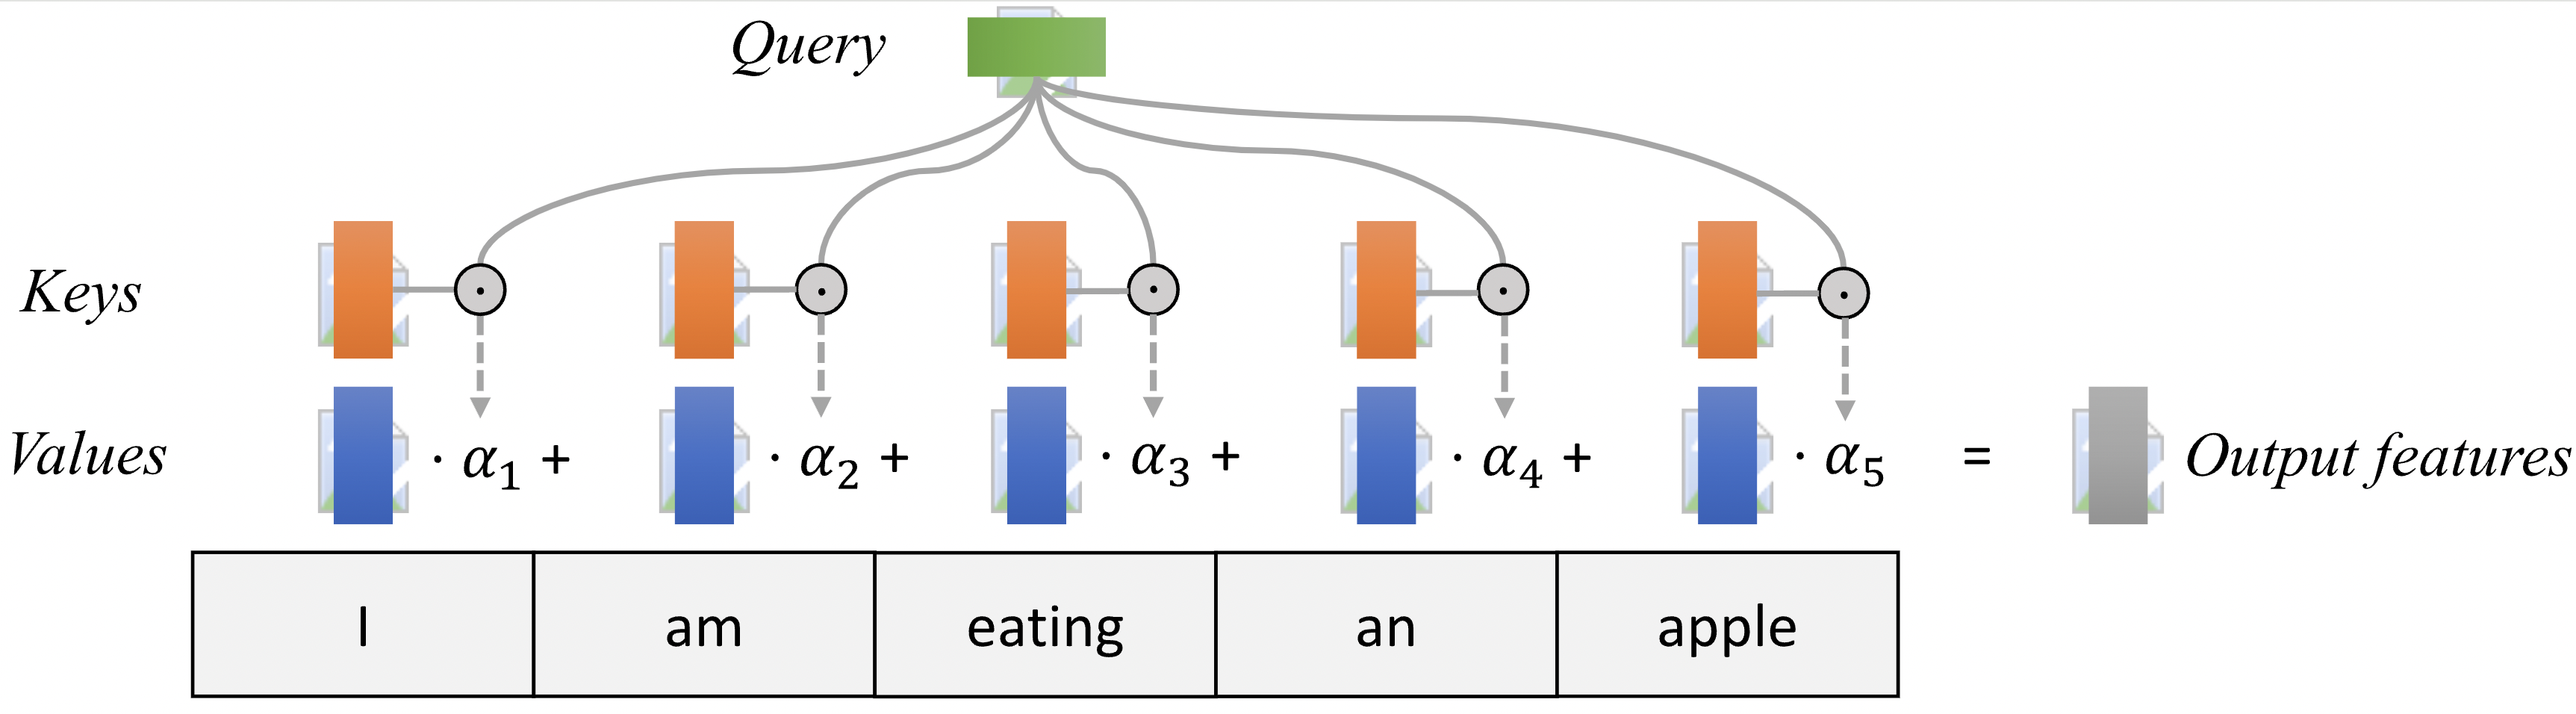
\includegraphics[scale=0.17,trim=0cm 0cm 0.6cm 0cm,clip=true]{figures/attention_example.png}
    % \caption{Caption}
    % \label{fig:enter-label}
\end{figure}




Most attention mechanisms differ in terms of what queries they use, how the key and value vectors are defined,
and what score function is used.
The attention applied inside the Transformer architecture is called \textbf{self-attention}.
In self-attention, each sequence element provides a key, value, and query.
For each element, we perform an attention layer where based on its query,
we check the similarity of all sequence elements' keys and returned a different,
averaged value vector for each element.
We will now go into a bit more detail by first looking at the specific implementation of the attention mechanism which is in the Transformer case the scaled dot product attention.

\subsubsection{Scaled Dot Product Attention}

The core concept behind self-attention is the scaled dot product attention.
Our goal is to have an attention mechanism with which any element in a sequence can attend to any other while
still being efficient to compute.
The dot product attention takes as input a set of queries
$Q\in\mathbb{R}^{T\times d_k}$, keys $K\in\mathbb{R}^{T\times d_k}$
and values $V\in\mathbb{R}^{T\times d_v}$ where $T$ is the sequence length,
and $d_k$ and $d_v$ are the hidden dimension for queries/keys and values respectively.
For simplicity, we neglect the batch dimension for now.
The attention value from element $i$ to $j$ is based on its similarity of the query $Q_i$ and key $K_j$,
using the dot product as the similarity metric.
In math, we calculate the dot product attention as follows:

$$\text{Attention}(Q,K,V)=\text{softmax}\left(\frac{QK^T}{\sqrt{d_k}}\right)V$$

The matrix multiplication $QK^T$ performs the dot product for every possible pair of queries and keys,
resulting in a matrix of the shape $T\times T$.
Each row represents the attention logits for a specific element $i$ to all other elements in the sequence.
On these, we apply a Softmax and multiply with the value vector to obtain a weighted mean
(the weights being determined by the attention).
Another perspective on this attention mechanism offers the computation graph which is visualized below (figure credit: \cite{vaswani2017attention}). There is also a nice visualization of these values are computed \href{https://miro.medium.com/v2/resize:fit:1973/1*G8thyDVqeD8WHim_QzjvFg.gif}{here}.

\begin{figure}[ht]
    \centering
    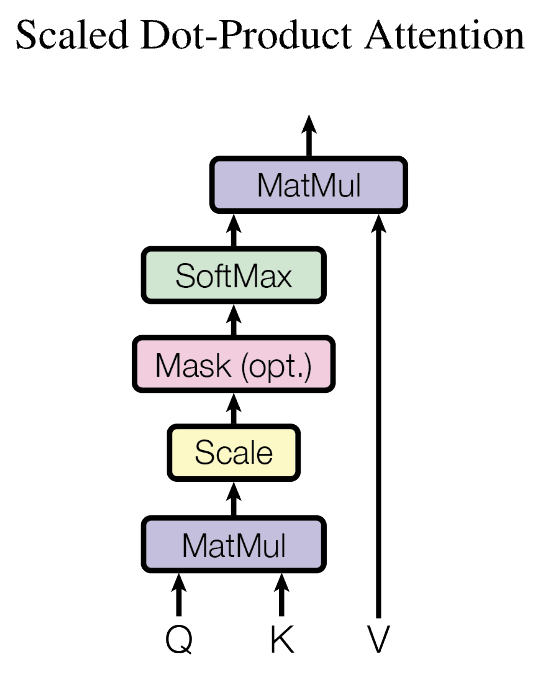
\includegraphics[scale=0.4]{figures/scaled_attention.png}
    % \caption{Caption}
    % \label{fig:enter-label}
\end{figure}



One aspect we haven't discussed yet is the scaling factor of $1/\sqrt{d_k}$.
This scaling factor is crucial to maintain an appropriate variance of attention values after initialization.
Remember that we initialize our layers to have equal variance throughout the model, and hence,
$Q$ and $K$ might also have a variance close to $1$.
However, performing a dot product over two vectors with a variance $\sigma$ results
in a scalar having $d_k$-times higher variance:

$$q_i \sim \mathcal{N}(0,\sigma), k_i \sim \mathcal{N}(0,\sigma) \to \text{Var}\left(\sum_{i=1}^{d_k} q_i\cdot k_i\right) = \sigma\cdot d_k$$


If we do not scale down the variance back to $\sigma$, the softmax over the logits will already saturate
to $1$ for one random element and $0$ for all others.
The gradients through the softmax will be close to zero so we can't learn the parameters appropriately.

\subsubsection{Multi-Head Attention}

The scaled dot product attention allows a network to attend over a sequence.
However, often there are multiple different aspects a sequence element wants to attend to,
and a single weighted average is not a good option for it.
This is why we extend the attention mechanisms to multiple heads,
i.e. multiple different query-key-value triplets on the same features.
Specifically, given a query, key, and value matrix, we transform those into $h$ sub-queries, sub-keys,
and sub-values, which we pass through the scaled dot product attention independently.
Afterward, we concatenate the heads and combine them with a final weight matrix.
Mathematically, we can express this operation as:


\begin{align}
    \text{Multihead}(Q,K,V) & = \text{Concat}(\text{head}_1,...,\text{head}_h)W^{O}\\
    \text{where } \text{head}_i & = \text{Attention}(QW_i^Q,KW_i^K, VW_i^V)
\end{align}


We refer to this as Multi-Head Attention layer with the learnable parameters
$W_{1...h}^{Q}\in\mathbb{R}^{D\times d_k}$,
$W_{1...h}^{K}\in\mathbb{R}^{D\times d_k}$,
$W_{1...h}^{V}\in\mathbb{R}^{D\times d_v}$,
and $W^{O}\in\mathbb{R}^{h\cdot d_k\times d_{out}}$ ($D$ being the input dimension).
Expressed in a computational graph, we can visualize it below
(figure credit: \cite{vaswani2017attention}).

\subsubsection{Causal Attention Masking}
For GPT-like LMs, we train the model to generate one token at a time from left to right (autoregressive). When predicting the next token, the autoregressive setup constraints the model to only ``see'', i.e. attend to, the preceding tokens on the left-hand side. For instance, given a sample training text: ``Life is short eat dessert first'', the self-attention should be applied only within the tokens on the left-hand side of the $\rightarrow$, in order to predict the token on the right-hand side:
\begin{itemize}
    \item ``Life'' $\rightarrow$ ``is''
    \item ``Life is'' $\rightarrow$ ``short''
    \item ``Life is short'' $\rightarrow$ ``eat''
    \item ``Life is short eat'' $\rightarrow$ ``dessert''
    \item ``Life is short eat dessert'' $\rightarrow$ ``first''
\end{itemize}

To achieve this in practice, one straightforward approach is to mask out future tokens for each timestamp by applying a mask to the attention weight matrix (causal attention masking). For the example above, we can apply the mask:
\begin{figure}[ht]
    \centering
    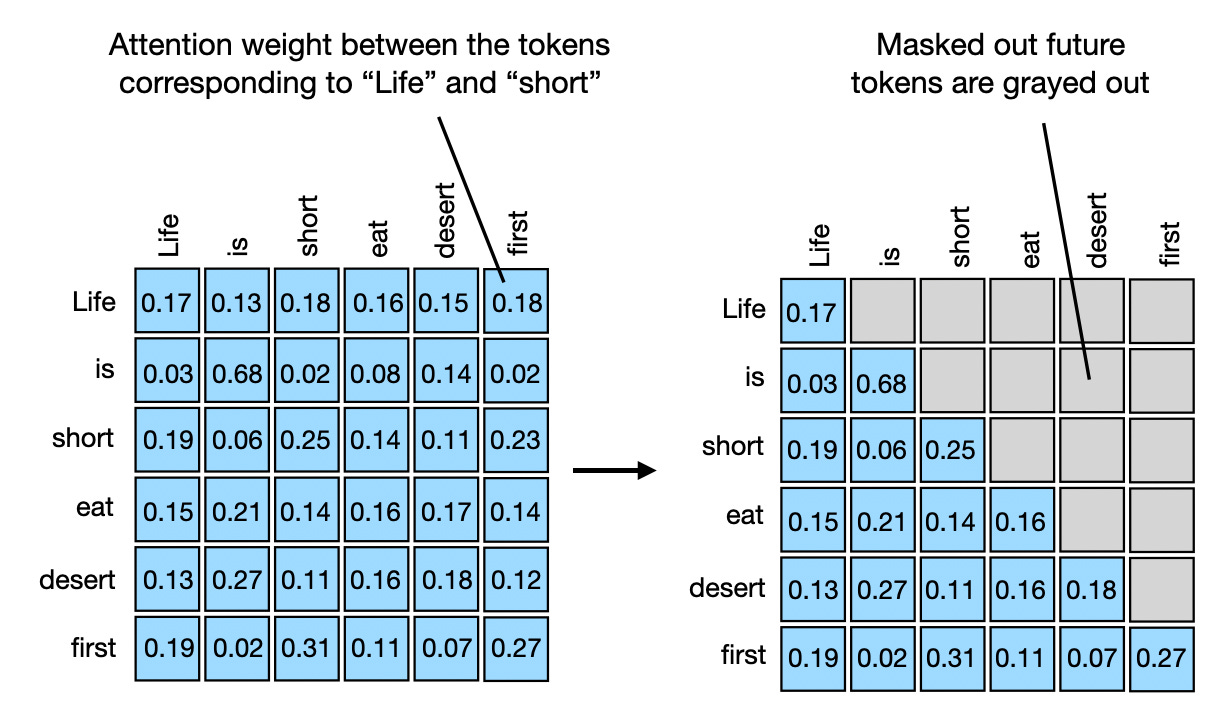
\includegraphics[scale=0.2]{figures/causal_attn_mask.jpg}
\end{figure}

\noindent\todo{}: Read and complete the missing lines in the \texttt{\_\_init\_\_} function of the \texttt{CausalSelfAttention} class in \texttt{gpt/model.py}, create the causal attention mask.\\
\noindent\textbf{Hint}: Follow the requirements and hints specified in the code comments.

\subsubsection{Putting it Together (so far): Multi-Head Self Attention with Causal Masking}
Now that we have delved into the details of all important components, it's time to build the causal self-attention block for our own GPT!\\

\noindent\todo{}: Read and complete the missing lines in the \texttt{forward} function of the \texttt{CausalSelfAttention} class in \texttt{gpt/model.py}.\\
\noindent\textbf{Hint}: Follow the requirements and hints specified in the code comments.


\subsubsection{Residual connection and normalization}
Notice that there is a residual connection and normalization on top of the multi-head attention layer.

\begin{figure}[ht]
    \centering
    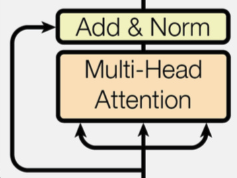
\includegraphics[scale=0.4]{figures/attn_residual.png}
    % \caption{Caption}
    % \label{fig:enter-label}
\end{figure}

Taking as input $x$, it is first passed through a Multi-Head Attention block as we have implemented above.
The output is added to the original input using a residual connection,
and we apply a consecutive Layer Normalization on the sum.
Overall, it calculates $\text{LayerNorm}(x+\text{Multihead}(x,x,x))$
($x$ being $Q$, $K$ and $V$ input to the attention layer).
The residual connection is crucial in the Transformer architecture for two reasons:

\begin{enumerate}
    \item Similar to ResNets, Transformers are designed to be very deep.
Some models contain more than 24 blocks in the encoder.
Hence, the residual connections are crucial for enabling a smooth gradient flow through the model.
    \item  Without the residual connection, the information about the original sequence is lost.
Remember that the Multi-Head Attention layer ignores the position of elements in a sequence,
and can only learn it based on the input features.
Removing the residual connections would mean that this information is lost after the first attention layer
(after initialization), and with a randomly initialized query and key vector,
the output vectors for position $i$ have no relation to its original input.
All outputs of the attention are likely to represent similar/same information,
and there is no chance for the model to distinguish which information came from which input element.
An alternative option to residual connection would be to fix at least one head to focus on its original input,
but this is very inefficient and does not have the benefit of the improved gradient flow.
\end{enumerate}

The Layer Normalization also plays an important role in the Transformer architecture as it enables faster
training and provides small regularization.
Additionally, it ensures that the features are in a similar magnitude among the elements in the sequence.
We are not using Batch Normalization because it depends on the batch size which is often small with Transformers
(they require a lot of GPU memory), and BatchNorm has shown to perform particularly badly in language
as the features of words tend to have a much higher variance (there are many, very rare words
which need to be considered for a good distribution estimate).


\subsubsection{Putting it Together: Transformer Architecture}

Originally, the Transformer model was designed for machine translation.
Hence, it has an encoder-decoder structure where the encoder takes as input the sentence in the original language and generates an attention-based representation. \textit{This is different from our GPT implementation, which is a decoder-only architecture.}
On the other hand, the decoder attends to the encoded information and generates the translated sentence in an auto-regressive manner, as in a standard RNN. The full Transformer architecture looks as follows
(figure credit: \cite{vaswani2017attention}):

\begin{figure}[h]
    \centering
    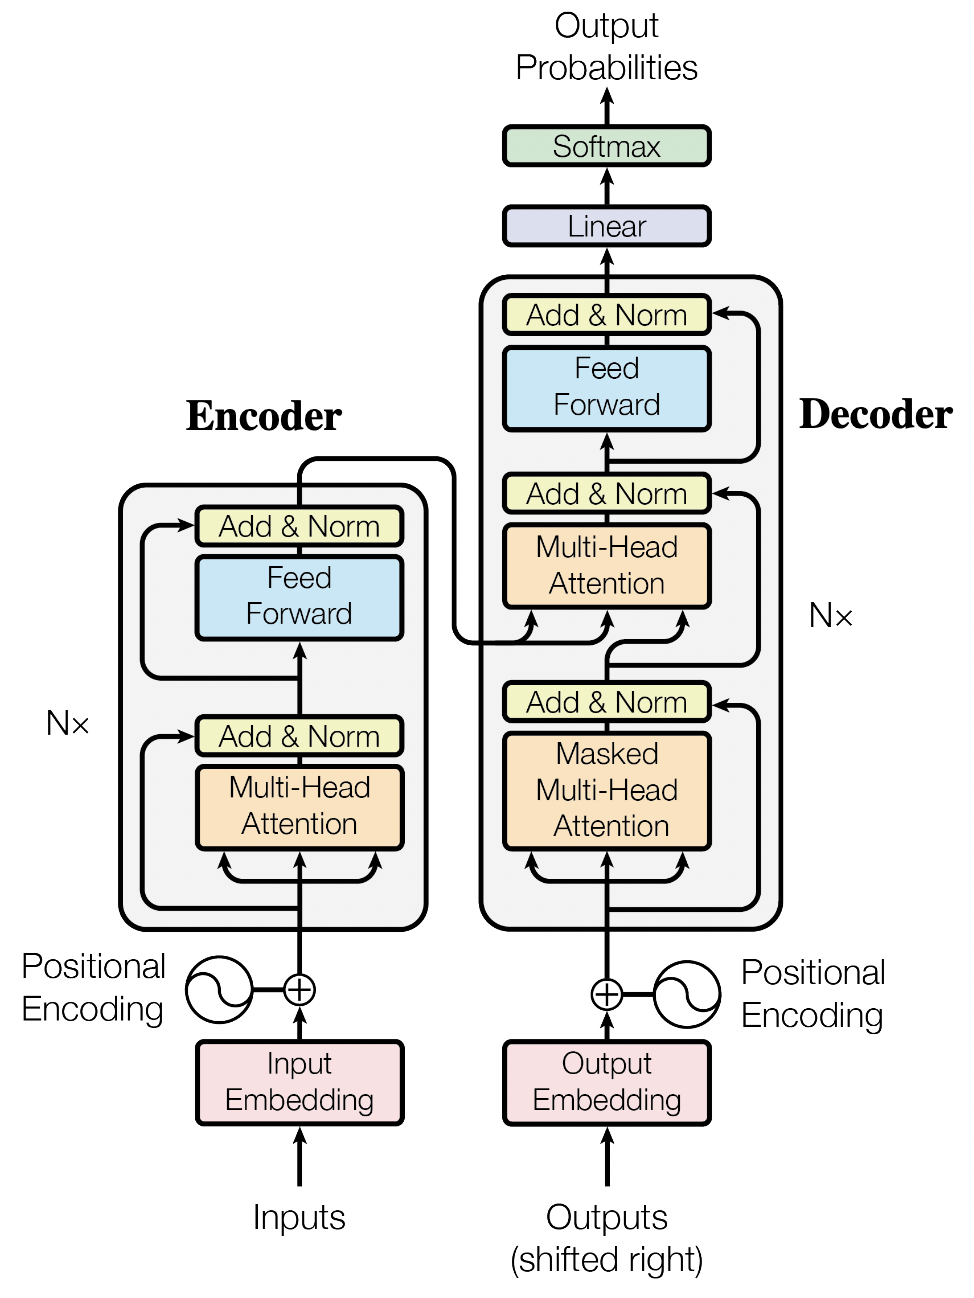
\includegraphics[scale=0.5]{figures/transformer.png}
    % \caption{Caption}
    % \label{fig:enter-label}
\end{figure}

The encoder consists of $N$ identical blocks. These blocks contain Self-Attention, Layer Normalization, and Residual connections. Additionally, a small fully connected feed-forward network is added to the model, which is applied to each position separately and identically.
Specifically, the model uses a Linear$\to$ReLU$\to$Linear MLP.
The full transformation including the residual connection can be expressed as:

\begin{align}
    \text{FFN}(x) & = \max(0, xW_1+b_1)W_2 + b_2\\
    x & = \text{LayerNorm}(x + \text{FFN}(x))
\end{align}


This MLP adds extra complexity to the model and allows transformations on each sequence element separately.
You can imagine as this allows the model to ``post-process'' the new information added by the previous Multi-Head Attention, and prepare it for the next attention block.
Usually, the inner dimension of the MLP is 2-8$\times$ larger than $d_{\text{model}}$,
i.e. the dimension of the original input $x$.
The general advantage of a wider layer instead of a narrow, multi-layer MLP is the faster, parallelizable execution.

\subsubsection{Train and Evaluate GPT LM on GPUs}
\label{subsubsec:gpu}
\noindent Now let's train our GPT LM!

From this homework on, we will be using GPUs. 
\noindent \textbf{Why GPUs?}
A crucial feature of PyTorch is the support of GPUs, short for Graphics Processing Unit. A GPU can perform many thousands of small operations in parallel, making it very well suitable for performing large matrix operations in neural networks. When comparing GPUs to CPUs, we can list the following \href{https://blogs.nvidia.com/blog/2009/12/16/whats-the-difference-between-a-cpu-and-a-gpu/}{main differences}:

CPUs and GPUs have both different advantages and disadvantages, which is why many computers contain both components and use them for different tasks. In case you are not familiar with GPUs, you can read up more details in this \href{https://blogs.nvidia.com/blog/2009/12/16/whats-the-difference-between-a-cpu-and-a-gpu/}{NVIDIA blog post} or \href{https://www.intel.com/content/www/us/en/products/docs/processors/what-is-a-gpu.html}{here}. 

GPUs can accelerate the training of your network up to a factor of $100$ which is essential for large neural networks. PyTorch implements a lot of functionality to support GPUs (mostly those of NVIDIA due to the libraries \href{https://developer.nvidia.com/cuda-zone}{CUDA} and \href{https://developer.nvidia.com/cudnn}{cuDNN}). 

To get a more direct comparison, let's run our model for 50 training steps with both CPU and GPU.\\

\noindent\todo{} Run the \texttt{cpu\_gpu\_comparison} in \texttt{main.py}, and fill in the running time below (will be printed out on the console):\\
\noindent\solution{\\
CPU - Trainer Time Elapsed: 50.22 seconds\\
GPU - Trainer Time Elapsed: 3.34 seconds
}
\\\\
\noindent Finally, let's run the full training and evaluation on GPU.\\

\noindent\todo{} Run the \texttt{gpu\_full\_run} function in \texttt{main.py} to train the GPT language model, paste the two generated plots here. This function will also sample from the trained GPT LM. paste the completion to the prefix after the plots.\\
\noindent {\color{red}{your plots}}\\
% uncomment the following lines to add your plots.
\begin{figure}[h]
    \centering
    \subfloat[train and dev loss of the GPT LM]{
        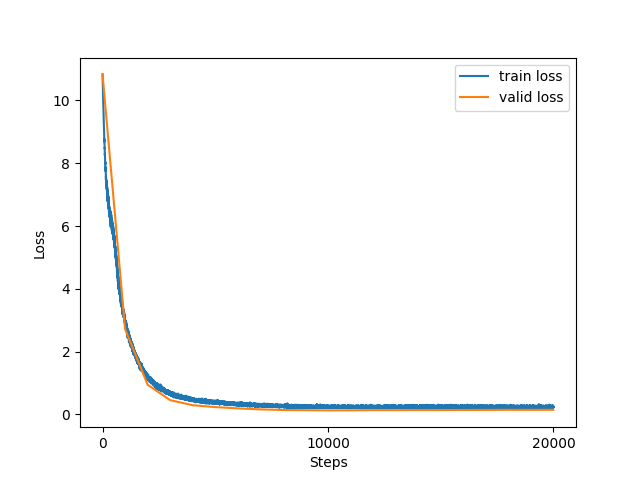
\includegraphics[width=0.45\textwidth]{figures/loss.png}
        }
    \hfill
    \subfloat[train and dev ppl of the MLP LM]{
        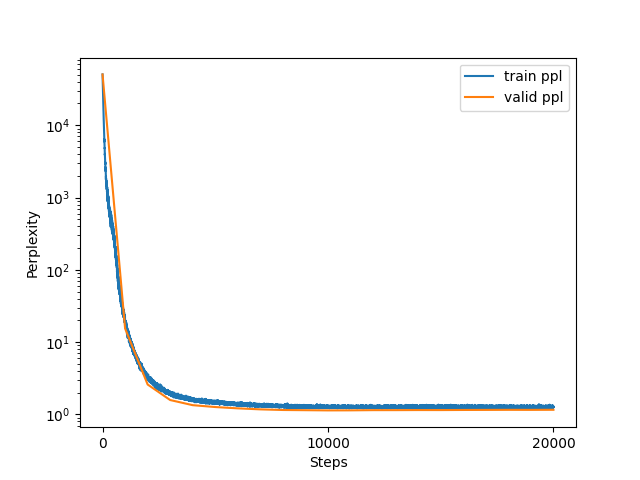
\includegraphics[width=0.45\textwidth]{figures/ppl.png}
        }
    \caption{loss and ppl of the GPT LM}
\end{figure}
\noindent\solution{\\
iter 20000: validation loss 0.14691 validation ppl 1.159\\
---------- Trainer Time Elapsed: 1228.19s ----------\\
--------------------------------------------------------------------------------\\
The best perks of living on the east east best best best best best best best best best best best best best best best best best best best beststicksIOIO best FreeBSD of living on the\\
--------------------------------------------------------------------------------\\
It is a truth universally acknowledged acknowledged acknowledged acknowledged acknowledged acknowledged acknowledged acknowledged acknowledged acknowledged acknowledged acknowledged acknowledged acknowledged acknowledged acknowledged acknowledged acknowledged acknowledged acknowledged acknowledged report vision vision too too acknowledged is a truth universally\\
--------------------------------------------------------------------------------\\
The best way to learn learn learn learn learn learn learn learn learn learn learn learn learn learn learn learn learn learn learn learn learn learn learn learn learn chance chance chance best way to\\
--------------------------------------------------------------------------------\\
According to the latest research research research research research to from from from from from from from from from from from from from from from from from research research research research from to the latest\\
}





\bibliographystyle{apalike}
\bibliography{ref}

\end{document}
